\documentclass[]{article}
\usepackage{graphicx}

%opening
\title{Parallellisme - Project report}
\author{Hans Van der Ougstraete}

\begin{document}

\maketitle
\clearpage
\tableofcontents
\clearpage

\section{Implementatie}

\subsection{Fase 1}
Fase 1 is opgedeeld in twee delen, het eerste deel maakt een lijst met relevante businesses door in de base case de evaluaterevalence methode uit SequentialSearch aan te roepen. De Yelpdata wordt dus in stukken opgedeeld tot het kleinste deel een business is. Deze lijst wordt in het tweede deel aan de hand van een parallele mergesort gesorteerd. Deze code is terug te vinden in de ParallelSearch klasse.
\subsection{Fase 2}
Het doorzoeken van de revieuw om het aantal voorkomens van een woord te bepalen kan op verschillende manieren.
Er bestaat een java klasse split welke een text opdeelt en per woord in een vector stopt. Echter heb ik moeilijkheden om de reguliere expressie die aangeeft waar een woord eindigt (bv spatie of leesteken) zo in te stellen dat de unit tests slagen. Ik had net iets meer of minder voorkomens dan de sequentiële search afhangende van de gebruikte reguliere expresie. Zonder controle over de input van de revieuws zou een reguliere expressie die voor een preset werkt misschien in een andere preset iets over het hoofd kijken. Deze code kan u vinden in CountOccurencesP en wordt aangeroepen in de functie countOccurencesP beide staan in ParallelSearch.java

Een ander oplossing is het gebruik van hashmaps, hierbij wordt het voorkomen van ieder woord geteld. Deze hash opslagen zou bij een volgende zoektocht snel het aantal voorkomens uit de hash kunnen halen. In deze hash zijn de woorden de key's en het aantal voorkomens de value.

Als derde oplossing heb ik geprobeerd de sequentiële manier van voorkomens tellen te parallelliseren. Het is me niet gelukt hier alle bugs uit te krijgen.
De code werkt omdat de tweede if-test in de compute functie altijd true is en het sequentiële algoritme start.
Deze code kan u vinden in CountOccurencesALT en wordt aangeroepen in de functie countOccurencesP beide staan in ParallelSearch.java


\section{Evaluatie}
De benchmarks op eigen computer (quad core i5-2300 @2.80GHz) zijn 4 maal uitgevoerd. Voor SequentialSearch, ParallelSearch met 1, 2 workers en ParallelSearch met 4 workers. Dit telkens 1500 keer. De resultaten worden per preset weergegeven.

\subsection{Fase 1}

\begin{figure}
	\centering
	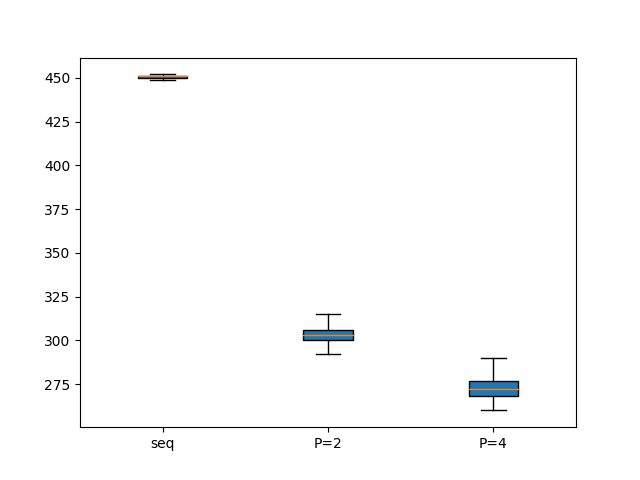
\includegraphics[width=0.7\linewidth]{Preset_1}
	\caption[Preset1]{Preset1}
	\label{fig:preset1}
\end{figure}

\begin{figure}
	\centering
	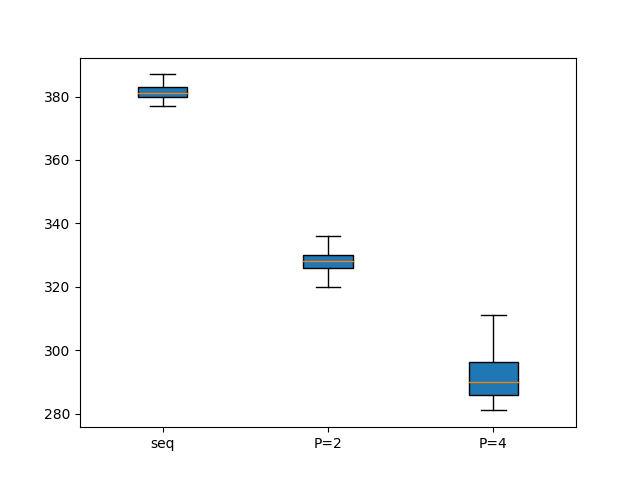
\includegraphics[width=0.7\linewidth]{Preset_2}
	\caption[Preset1]{Preset2}
	\label{fig:preset2}
\end{figure}

\begin{figure}
	\centering
	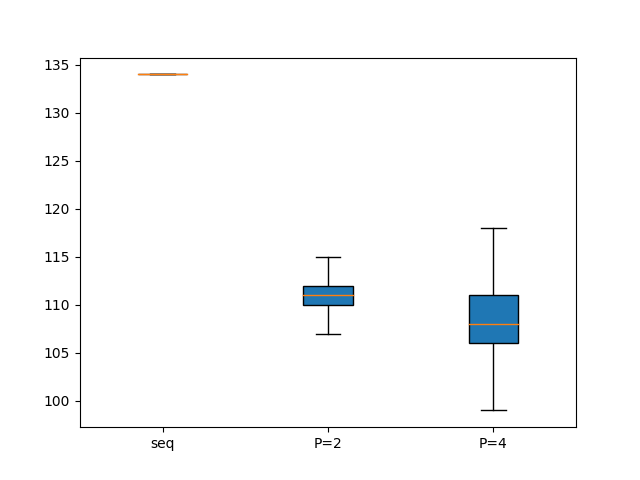
\includegraphics[width=0.7\linewidth]{Preset_3}
	\caption[Preset1]{Preset3}
	\label{fig:preset3}
\end{figure}

\begin{table}[h!]
	\centering
	\begin{tabular}{|c|c|c|c|}
		\hline 
		Runtime ms & Preset1 & Preset2 & Preset3 \\ 
		\hline 
		Parallel P=1 & 466 & 514 & 145 \\ 
		\hline 
		Parallel P=2 & 304 & 328 & 111 \\ 
		\hline 
		Parallel P=4 & 273 & 291 & 108 \\ 
		\hline 
		Sequential & 451 & 381 & 134 \\ 
		\hline 
	\end{tabular}
	\caption{Gemiddele runtime in miliseconden}
	\label{table:1}
\end{table}

\subsubsection{Overhead}

\begin{table}[h!]
	\centering
\begin{tabular}{|c|c|c|c|}
	\hline 
	Overhead & Preset1 & Preset2 & Preset3 \\ 
	\hline 
	T1/Tseq & 1.03 & 1.35 & 1.08 \\ 
	\hline 
\end{tabular} 
\caption{Overhead waarden voor de 3 presets.}
\label{table:2}
\end{table}

Bovenstaande tabel toont de overhead, deze overhead van het verdelen in threads is niet aanwezig bij de sequentiële versie omdat de sequentiële versie niet opdeelt in alsmaar kleinere taken. De overhead is verschillend per preset omdat het opdelen van het werk afhangt van de respectievelijke data.
De overhead kan kleiner gemaakt worden door een goede cut-off waarde te gebruiken, hierdoor wordt er sneller sequentieel gewerkt en daardoor minder opgedeeld in subtaken.

\subsubsection{Speed-up}
\begin{table}[h!]
	\centering
	\begin{tabular}{|c|c|c|c|}
		\hline 
		Speed-up & Preset1 & Preset2 & Preset3 \\ 
		\hline 
		Tseq/T2 & 1.48 & 1.16 & 1.21 \\ 
		\hline 
		Tseq/T4 & 1.65 & 1.31 & 1.24 \\ 
		\hline 
	\end{tabular} 
	\caption{Speed-up values for all 3 presets.}
	\label{table:2}
\end{table}

Een perfecte speed-up zou gelijk zijn aan het aantal extra processors, dit is hier niet het geval.
De speed-up is ook verschillend per preset, het aantal businesses en revieuws beïnvloeden dit volgens mij.
Bij preset 3 is er nauwelijks verschil tussen T=2 en T=4, ik veronderstel dat dit is omdat de data klein is.
het meeste winst wordt geboekt bij preset 1, de preset met het meest aantal businesses.

\subsection{Fase 2}

Hoewel de eerste manier (a.d.h.v split functie) werkt op mijn laptop en het aantal voorkomens parallel wordt geteld, werkt deze spijtig genoeg niet op serenity. De alternatieve versie draait maar telt de voorkomens niet parallel. Hierdoor kan ik niet expliciet testen met verschillende cutoff waardes.

Ik heb hierdoor geen metingen voor verschillende threshold's van T. De beste waarde voor T zou een waarde zijn die de overhead minimaliseert en de beste snelheid winst geeft. Een te hoge waarde voor T resulteert in te veel sequentieel werkt terwijl een te lage waarde zou de overhead onnodig groot maakt. Bij een te lage waarde T zou er meer tijd verloren gaan in het maken van al de taken en hierdoor geen snelheidswinst meer gemeten worden.

De onderstaande resultaten werden bekomen door een jar file van het project te laten lopen. Deze neemt 4 argumenten, P, T, DataPreset en het aantal keer dat de file uitgevoerd moet worden. De resultaten van zo een testrun worden weggeschreven naar een csv file. Praktisch heb ik een script aangemaakt dat de test 30 maal uitvoerde voor P waardes 1,4,8,16,32,64. Hierbij verdubbeld het aantal cores bij elke volgende test.
De verkregen csv files heb ik dan lokaal gekopieerd, de waarden gesorteerd en telkens de mediaan geselecteerd om de speed-up te berekenen. De exacte code voor het verloop van de test staat in de main functie van het project. 
\subsubsection{Speed-up}
De testen werden telkens 30 keer uitgevoerd voor 4, 8, 16, 32 en 64 processors.
De berekening voor de speed-up is uitgevoerd met de mediaan uit de testresultaten. 

\begin{table}[h!]
	\centering
	\begin{tabular}{|c|c|}
		\hline 
		Speed-up & Preset1 \\ 
		\hline 
		T1/T4 & 1.75 \\ 
		\hline 
		T1/T8 & 2.03 \\ 
		\hline 
		T1/T16 & 1.98 \\ 
		\hline
		T1/T32 & 2.10 \\ 
		\hline
		T1/T64 & 2.09 \\ 
		\hline
	\end{tabular} 
	\caption{Speed-up values on serenity.}
	\label{table:3}
\end{table}

\subsection{Conclusie}
In bovenstaande tabel kunnen we zien dat de code vanaf 8 processors niet veel snelheidswinst boekt.
Volgens mij is de oorzaak het sequentiële deel van de code, namelijk het doorzoeken van de reviews dat hier een bottleneck vormt om de performantie te kunnen verhogen zou dit ook parallel moeten gebeuren met een ideale T zodat de overhead klein blijft. 
De work en de span worden eigenlijk gedefinieerd door de dag van de parallelle reductie.
Waar work O(n) is en de span O(log n), uit de test met P=1 leidt ik af dat gemiddelde gemeten waarde voor work 2,9 seconden of 173500 milliseconden is. aan de hand van deze T1 kunnen we de speed-up berekenen voor meerdere processors. Als we de speed-up van Preset1 op eigen computer vergelijken met de testen op serenity, telkens voor P=4 zien we een gelijkaardige speed-up. Wat we op serenity niet vergelijken zijn speed-ups op verschillende data. Afgeleid uit de waarden uit de tests op eigen computer kunnen hier grote verschillen ontstaan.

\end{document}
